% ============================================================
%  Astera Labs 全面调研报告 — Part 1-3
%  编译引擎：XeLaTeX
%  日期：2026-05-19
% ============================================================

\documentclass[UTF8,11pt,aspectratio=169]{beamer}
\usepackage{xeCJK}
\setCJKmainfont{Songti SC}
\setCJKsansfont{Heiti SC}
\setCJKmonofont{STFangsong}

\usetheme{Darmstadt}
\usecolortheme{whale}
\usefonttheme{professionalfonts}

\definecolor{darkgreen}{RGB}{0,128,0}
\definecolor{darkred}{RGB}{180,0,0}
\definecolor{darkblue}{RGB}{0,0,139}
\definecolor{gold}{RGB}{200,150,0}
\definecolor{mygray}{RGB}{245,245,245}
\definecolor{t1green}{RGB}{220,255,220}
\definecolor{t2blue}{RGB}{200,220,255}
\definecolor{t3yellow}{RGB}{255,255,200}
\definecolor{t4orange}{RGB}{255,230,200}
\definecolor{t5red}{RGB}{255,200,200}

\usepackage{graphicx}
\usepackage{tikz}
\usetikzlibrary{positioning, calc, shapes.geometric, arrows.meta, backgrounds, fit, chains}
\usepackage{booktabs}
\usepackage{tabularx}
\usepackage{multirow}
\usepackage{array}
\usepackage[table]{xcolor}
\usepackage{amsmath,amssymb}
\usepackage{mathtools}
\usepackage{listings}
\usepackage{hyperref}
\hypersetup{colorlinks=true, linkcolor=darkblue, urlcolor=darkblue}
\usepackage{bookmark}
\usepackage{pgfpages}

\lstset{
    basicstyle=\ttfamily\small,
    keywordstyle=\color{blue}\bfseries,
    commentstyle=\color{darkgreen},
    stringstyle=\color{darkred},
    numbers=left,
    numberstyle=\tiny\color{gray},
    backgroundcolor=\color{mygray},
    breaklines=true,
    frame=single,
    tabsize=2
}

\title[Astera Labs 全面调研]{Astera Labs 全面调研报告}
\subtitle{工程级别、产业级别的深度分析}
\author[Ge Liangchen]{Ge Liangchen}
\date{\today}
\institute{半导体行业分析}

\setbeamertemplate{footline}[frame number]

\AtBeginSection[]{
    \begin{frame}{目录}
        \tableofcontents[currentsection]
    \end{frame}
}

% ---- 自定义命令 ----
\newcommand{\sourceT}[1]{{\small\textcolor{darkblue}{[T#1]}}}
\newcommand{\unverified}{{\textcolor{darkred}{\textbf{[未确认]}}}}
\newcommand{\speculation}{{\textcolor{orange}{\textbf{[推测]}}}}
\newcommand{\marketing}{{\textcolor{orange}{\textbf{[可能为营销语言]}}}}

\begin{document}

\begin{frame}
    \titlepage
\end{frame}

\begin{frame}{报告结构总览}
    \tableofcontents
\end{frame}

% ============================================================
%  PART 1：公司整体定位
% ============================================================
\section{Part 1: 公司整体定位}

\begin{frame}{公司基本信息}
    \begin{table}
        \caption{Astera Labs 公司概览}
        \begin{tabular}{lll}
            \toprule
            \textbf{属性} & \textbf{内容} & \textbf{来源} \\
            \midrule
            公司全称 & Astera Labs, Inc. & \sourceT{1} SEC \\
            成立时间 & 2017年 & \sourceT{2} Wikipedia \\
            总部 & Santa Clara, CA → 2025年迁至San Jose & \sourceT{2} Wikipedia \\
            上市时间 & 2024年3月 (Nasdaq: ALAB) & \sourceT{1} SEC \\
            IPO定价 & 约\$5.5B估值, 募资\$713M & \sourceT{2} Wikipedia \\
            商业模式 & Fabless (无晶圆厂) & \sourceT{2} 官方 \\
            晶圆代工 & TSMC & \sourceT{3} SemiAnalysis \\
            员工规模 & 未公开精确数字 & \unverified \\
            行业分类 & SIC 3674 (Semiconductors \& Related Devices) & \sourceT{1} SEC \\
            \bottomrule
        \end{tabular}
    \end{table}
\end{frame}

\note{
    创始人背景（来源[T2] Wikipedia）：
    - Jitendra Mohan (CEO): 前Texas Instruments高管
    - Sanjay Gajendra: 前Texas Instruments
    - Casey Morrison: 前Texas Instruments
    三人在TI共事后，观察到数据中心连接技术未能跟上AI/ML的发展步伐，在Sanjay Gajendra的车库中开始创业。

    融资历史（来源[T2] Wikipedia, [T3] SemiAnalysis）：
    - Series B (2020年4月): Avigdor Willenz, Intel Capital, Ron Jankov, Sutter Hill Ventures
    - Series C (2021年9月): \$50M, Fidelity领投，估值约\$950M
    - Series D (2022年11月): \$150M，估值超过\$3B
    - 曾拒绝Marvell的收购要约（来源[T3] SemiAnalysis）
    - IPO underwriters: Morgan Stanley, JPMorgan
}

\begin{frame}{创始团队与关键人物}
    \begin{columns}[T]
        \begin{column}{0.5\textwidth}
            \textbf{创始人} \sourceT{2}：
            \begin{itemize}
                \item \textbf{Jitendra Mohan} — CEO
                \item \textbf{Sanjay Gajendra}
                \item \textbf{Casey Morrison}
            \end{itemize}
            \vspace{0.3cm}
            三人均来自 \textbf{Texas Instruments}
        \end{column}
        \begin{column}{0.5\textwidth}
            \textbf{当前高管（来自官网/博客）} \sourceT{2}：
            \begin{itemize}
                \item Thad Omura — SVP \& GM, Compute Connectivity
                \item Amit Golander, PhD — AVP, Memory \& Storage
                \item Jignesh Shah — Sr. Director, Signal Connectivity
                \item Caleb Shetland — Sr. Principal, Firmware
                \item Mike Hendricks — AVP, Solutions \& Ecosystem
            \end{itemize}
        \end{column}
    \end{columns}

    \vspace{0.3cm}
    \begin{keypoint}
        TI 背景意味着创始团队对模拟/混合信号设计有深厚积累 —— 这正是高速SerDes/Retimer的核心能力。
    \end{keypoint}
\end{frame}

\note{
    创始团队三人全部来自TI，这一点对理解Astera Labs的技术护城河非常重要。TI是全球模拟和混合信号芯片的领导者，其工程师在SerDes、PLL、信号完整性等高速模拟设计领域有深厚的积累。Retimer本质上是一个高速模拟/DSP混合信号产品，TI背景恰好匹配。

    此外，Intel Capital作为早期投资方也值得注意。Intel是PCIe和CXL标准的主要推动者之一，这个关系可能对Astera Labs的产品路线图提供了标准层面的前瞻性指导。
}

\begin{frame}{公司核心定位}
    \centering
    \begin{tikzpicture}[
        box/.style={rectangle, draw=darkblue, fill=blue!5, thick, minimum width=4cm, minimum height=1.2cm, align=center, rounded corners=5pt},
        arrow/.style={->, >=Stealth, thick}
    ]
        \node[box, fill=darkred!10] (SLOGAN) at (0,0) {\textbf{"Purpose-Built Connectivity}\\\textbf{for Rack-Scale AI"}};
        \node[box, fill=darkgreen!10, below=0.8cm of SLOGAN] (POS) {\textbf{定位：AI Infra 连接层供应商}};
        \node[box, fill=yellow!10, below=0.8cm of POS] (DIFF) {\textbf{差异化：Open Standards}\\(PCIe/CXL vs 私有NVLink)};
    \end{tikzpicture}

    \vspace{0.5cm}
    \begin{columns}[T]
        \begin{column}{0.33\textwidth}
            \begin{block}{核心问题}
                AI服务器内部的GPU-to-GPU、GPU-to-memory、GPU-to-NIC连接是瓶颈
            \end{block}
        \end{column}
        \begin{column}{0.33\textwidth}
            \begin{block}{解决方案}
                提供完整的信号调理+交换+内存+软件平台
            \end{block}
        \end{column}
        \begin{column}{0.33\textwidth}
            \begin{block}{商业逻辑}
                Hyperscaler需要独立于NVIDIA的连接方案
            \end{block}
        \end{column}
    \end{columns}
\end{frame}

\note{
    Astera Labs的核心定位可以总结为三个层次：
    1. 物理层：通过Aries Retimer/Cable Module解决高速信号传输问题
    2. 架构层：通过Scorpio Fabric Switch解决GPU/NIC/Storage之间的交换互连问题
    3. 系统层：通过COSMOS提供全链路的telemetry和fleet management

    这三个层次构成了一个完整的"连接平台"——从铜线到软件管理。

    关键的商业逻辑：hyperscaler（AWS、Google、Microsoft、Meta等）不希望完全绑定NVIDIA的专有网络（NVLink/NVSwitch），他们需要基于开放标准（PCIe/CXL）的替代方案来保持供应商多样性和议价能力。
}

\begin{frame}{产业链位置}
    \centering
    \begin{tikzpicture}[
        node distance=2.2cm and 1.5cm,
        box/.style={rectangle, draw=darkblue, thick, minimum width=2.5cm, minimum height=1cm, align=center, rounded corners=3pt},
        arrow/.style={->, >=Stealth, thick},
        highlight/.style={rectangle, draw=darkred, fill=red!10, thick, minimum width=2.8cm, minimum height=1cm, align=center, rounded corners=3pt}
    ]
        % Upstream
        \node[box, fill=gray!10] (EDA) {EDA/IP\\Synopsys/Cadence};
        \node[box, fill=gray!10, right=of EDA] (FAB) {晶圆代工\\TSMC};
        \node[box, fill=gray!10, right=of FAB] (OSAT) {封装测试\\OSAT};

        % Astera
        \node[highlight, below=of FAB] (AST) {\textbf{Astera Labs}\\\textbf{Fabless Chip Designer}};

        % Products
        \node[box, fill=blue!5, below left=of AST] (P1) {Scorpio\\Fabric Switch};
        \node[box, fill=blue!5, below=of AST] (P2) {Aries\\Retimer/Cable};
        \node[box, fill=blue!5, below right=of AST] (P3) {Leo/Taurus\\CXL/Ethernet};

        % Customers
        \node[box, fill=darkgreen!10, below=of P2, minimum width=3cm] (CUST) {Hyperscalers\\+ Server OEM + GPU Vendor};

        % Arrows
        \draw[arrow] (EDA) -- (AST);
        \draw[arrow] (FAB) -- (AST);
        \draw[arrow] (OSAT) -- (AST);
        \draw[arrow] (AST) -- (P1);
        \draw[arrow] (AST) -- (P2);
        \draw[arrow] (AST) -- (P3);
        \draw[arrow] (P1) -- (CUST);
        \draw[arrow] (P2) -- (CUST);
        \draw[arrow] (P3) -- (CUST);
    \end{tikzpicture}

    \vspace{0.3cm}
    \textbf{供应链结构} \sourceT{3}：Fabless设计 → TSMC代工 → OSAT封测 → 供货给hyperscaler/OEM
\end{frame}

\begin{frame}{核心概念解释 (1)}
    \begin{block}{Rack-Scale AI}
        \begin{itemize}
            \item \textbf{含义}：单个AI服务器已无法容纳所需GPU数量，多个服务器需跨机架（rack）协同工作
            \item \textbf{为何重要}：GPT-4级别模型训练需要数千GPU互连；推理大模型也需要多GPU
            \item \textbf{连接挑战}：机架内的GPU间需要极高带宽、极低延迟的连接；跨机架需要更长距离（>3m）的高速连接
        \end{itemize}
    \end{block}

    \vspace{0.2cm}
    \begin{block}{Scale-Up Fabric vs Scale-Out Network}
        \begin{itemize}
            \item \textbf{Scale-Up Fabric}：服务器/机架内部，GPU-to-GPU，追求超低延迟、超高带宽（如NVLink、Scorpio X-Series），通常\<10m
            \item \textbf{Scale-Out Network}：跨机架/跨集群，Node-to-Node，关注带宽和扩展性（如InfiniBand、Ethernet），距离可达100m+
        \end{itemize}
    \end{block}
\end{frame}

\note{
    Rack-Scale AI 的核心驱动因素：
    - AI模型规模每18-24个月增长10x（比摩尔定律更快）
    - 单个GPU的HBM容量（如H100 80GB, H200 141GB, B200 192GB）远小于模型需要的内存量（GPT-4约1.76T参数需要>3.5TB内存用于推理）
    - 因此GPU必须互连，形成逻辑上的"大GPU"
    - 连接带宽决定GPU利用率——如果连接慢，GPU就空闲等待数据

    Scale-Up vs Scale-Out:
    - Scale-Up = 让一个"系统"更大（更多GPU在一个coherent域内）
    - Scale-Out = 让更多"系统"并行工作（每个系统独立，通过网络通信）
    - NVLink (900 GB/s per GPU) vs InfiniBand (400 GB/s per port)

    Astera Labs 的定位恰好在这两者的交汇处：
    - Scorpio X-Series 瞄准 scale-up（替代/补充NVSwitch）
    - Scorpio P-Series 瞄准 I/O 连接（GPU-to-NIC-to-Storage）
    - Aries Cable 连接这两个域
}

\begin{frame}{核心概念解释 (2)}
    \begin{block}{PCIe Fabric}
        \begin{itemize}
            \item \textbf{含义}：用PCIe交换机将多个设备（GPU、NIC、NVMe、CPU）连接成一个可灵活拓扑的"fabric"网络
            \item \textbf{vs 传统PCIe树}：传统PCIe是树形拓扑（CPU为根），Fabric支持mesh/torus等更灵活拓扑
            \item \textbf{Astera的角色}：Scorpio系列是专门为AI优化的PCIe Fabric Switch
        \end{itemize}
    \end{block}

    \vspace{0.2cm}
    \begin{block}{CXL Fabric 与 Memory Semantic Interconnect}
        \begin{itemize}
            \item \textbf{CXL} = Compute Express Link，基于PCIe物理层构建的缓存一致性互连协议
            \item \textbf{Memory Semantic}：不只是DMA传输数据块，而是像访问本地内存一样进行load/store操作
            \item \textbf{CXL Fabric}：用CXL交换机将多个host连接到共享的内存池
            \item \textbf{为何AI需要}：AI模型太大装不进单一GPU的HBM → 需要更大但成本更低的DDR内存池
        \end{itemize}
    \end{block}
\end{frame}

\note{
    关键区分——PCIe Fabric vs CXL Fabric:
    - PCIe Fabric: 用于连接I/O设备（GPU、NIC、NVMe），数据传输以DMA/TLP为主，是非coherent的
    - CXL Fabric: 基于PCIe电气层但运行CXL协议，支持cache coherency，可以做load/store语义的内存访问
    - 两者运行在同一PCB/连接器上但跑不同协议——这对理解Scorpio为什么能同时支持PCIe和"memory semantic"至关重要

    "Memory Semantic"的真实含义：
    - 传统PCIe设备只能通过DMA方式访问内存，需要软件介入
    - CXL允许CPU/GPU通过load/store指令直接访问远端内存（像NUMA一样）
    - 这就是"semantic"——访问方式从"发消息"变成了"直接读/写内存地址"
    - 延迟仍然比本地DRAM高（+200ns级别），但比走网络的RDMA（微秒级）低得多
}

\begin{frame}{竞争生态图}
    \centering
    \begin{tikzpicture}[
        node distance=1.2cm and 1cm,
        layer/.style={rectangle, draw=darkblue, fill=blue!5, thick, minimum width=3.5cm, minimum height=0.7cm, align=center},
        comp/.style={rectangle, draw=darkred, fill=red!5, thick, minimum width=2cm, minimum height=0.7cm, align=center, font=\footnotesize},
        collab/.style={rectangle, draw=darkgreen, fill=green!5, thick, minimum width=2cm, minimum height=0.7cm, align=center, font=\footnotesize},
        ast/.style={rectangle, draw=gold, fill=yellow!10, very thick, minimum width=2.2cm, minimum height=0.8cm, align=center, font=\footnotesize\bfseries}
    ]
        % Layers
        \node[layer] (L1) {PCIe Retimer / Cable Module};
        \node[layer, below=0.3cm of L1] (L2) {PCIe Fabric Switch};
        \node[layer, below=0.3cm of L2] (L3) {CXL Memory Controller};
        \node[layer, below=0.3cm of L3] (L4) {Ethernet Cable Module};
        \node[layer, below=0.3cm of L4] (L5) {Software / Fleet Mgmt};

        % Competitors per layer
        \node[comp, right=0.5cm of L1] {Broadcom\\Credo\\Parade\\Renesas};
        \node[comp, right=0.5cm of L2] {Broadcom (PEX)\\Microchip (Switchtec)};
        \node[comp, right=0.5cm of L3] {Samsung\\SK hynix\\Micron\\Montage};
        \node[comp, right=0.5cm of L4] {Credo\\Broadcom\\Marvell};
        \node[comp, right=0.5cm of L5] {NVIDIA (NVLink Mgmt)\\各BMC厂商};

        % Astera position
        \node[ast, left=0.5cm of L1, minimum height=3.8cm] (ASTERA) {Astera Labs\\\vspace{0.1cm}\\全栈覆盖};

        % Partners
        \node[collab, below right=0.3cm and 0.3cm of L5] (NVIDIA) {NVIDIA (GTC合作)};
        \node[collab, right=of NVIDIA] (ARM) {Arm (Total Design)};
        \node[collab, right=of ARM] (INTEL) {Intel (CXL互操作)};

        % Arrows
        \draw[->, thick] (ASTERA.east) -- (L1.west);
        \draw[->, thick] (ASTERA.east) -- (L2.west);
        \draw[->, thick] (ASTERA.east) -- (L3.west);
    \end{tikzpicture}

    \begin{keypoint}
        Astera Labs 是唯一一家横跨 PCIe Retimer + PCIe Switch + CXL Controller + Ethernet + 软件管理平台的连接件公司。
        其主要竞争对手（Broadcom、Credo、Microchip等）通常只在其中1-2层竞争。
    \end{keypoint}
\end{frame}

\note{
    竞争格局的详细分析见 Part 8。

    核心竞争优势（从生态图可看出）：
    - "全栈"不是简单的产品组合，而是通过COSMOS软件平台将物理层到系统层的telemetry统一管理
    - 对hyperscaler而言："one throat to choke" —— 一个供应商覆盖所有连接需求
    - 对Broadcom而言：Astera正在从Retimer向上扩展到Switch（这是Broadcom的核心领地）
    - 对NVIDIA而言：Astera提供了基于开放标准的替代方案，帮助客户避免NVLink锁定

    "Switzerland of connectivity" 的含义：
    - 类比：瑞士在二战中的中立地位
    - Astera不卖GPU，不卖CPU，不卖服务器——只做连接
    - 因此可以和所有厂商合作（Intel/AMD CPU + NVIDIA/AMD GPU + 各种NIC/Storage）
    - NVIDIA的NVSwitch是"只连NVIDIA GPU的私有方案"，而Scorpio连接任何PCIe设备
}

\begin{frame}{为什么Hyperscaler需要独立Connectivity Vendor}
    \begin{enumerate}
        \item \textbf{避免NVIDIA锁定}：NVLink/NVSwitch是私有协议，仅NVIDIA GPU能用。Hyperscaler需要基于PCIe/CXL开放标准的替代方案来保持多GPU供应商策略
        \item \textbf{统一管理平面}：不同设备（GPU/NIC/NVMe）的连接如果在不同供应商手上，管理和调试极度困难。COSMOS提供统一telemetry
        \item \textbf{custom需求}：Hyperscaler需要定制化的拓扑而非标准服务器设计，传统芯片公司（Broadcom）未必愿意定制
        \item \textbf{信号完整性挑战}：PCIe 6 PAM4时代，从芯片到cable到背板的SI挑战呈指数增长，需要深度know-how
    \end{enumerate}

    \begin{alertblock}{关键洞察}
        NVIDIA的NVSwitch生态越强大，hyperscaler对开放替代方案的需求就越强烈。Astera Labs的价值与NVIDIA的垄断程度正相关。
    \end{alertblock}
\end{frame}

\note{
    关于"NVIDIA锁定"的深层逻辑：
    - H100/B200等GPU的NVLink端口只能连NVSwitch或同型号GPU
    - 如果hyperscaler想要混合使用NVIDIA GPU和AMD GPU、或自研ASIC（如Google TPU、Amazon Trainium），NVSwitch无法提供服务
    - PCIe作为行业标准，任何设备都支持
    - 所以Astera的目标市场是：(1)非NVIDIA GPU互连 (2)异构计算环境 (3)NVIDIA GPU的非NVLink侧I/O扩展

    关于"独立vendor"的持久性：
    - 如果Astera成功到一定程度，Broadcom或NVIDIA可能通过并购或产品扩展来竞争
    - 但hyperscaler偏好多供应商，所以即使Broadcom有类似产品，hyperscaler也会保留Astera作为second source
    - "中立性"是一种真实但脆弱的护城河——取决于竞争格局的变化速度
}

% ============================================================
%  PART 2：产品线全景
% ============================================================
\section{Part 2: 产品线全景}

\begin{frame}{产品线总览}
    \begin{table}
        \caption{Astera Labs 全产品线}
        \begin{tabular}{lllp{0.3\textwidth}}
            \toprule
            \textbf{产品} & \textbf{类型} & \textbf{协议} & \textbf{核心价值} \\
            \midrule
            \rowcolor{blue!5}
            Scorpio X-Series & Fabric Switch & Memory Semantic & GPU Scale-Up Fabric, 320 lanes \\
            \rowcolor{blue!5}
            Scorpio P-Series & Fabric Switch & PCIe 6 & PCIe Fabric, 32-320 lanes \\
            \midrule
            Aries Retimer & Signal Conditioning & PCIe 6/CXL & 信号再生, DSP均衡 \\
            Aries Smart Cable & Active Cable Module & PCIe 6/CXL & 7m铜缆, 64GT/s \\
            Aries Gearbox & Protocol Bridge & PCIe 6→5 & PCIe代际过渡 \\
            \midrule
            Leo & Memory Controller & CXL 1.1 & DDR5内存扩展/池化 \\
            \midrule
            Taurus & Active Cable Module & Ethernet & 800G, 7m \\
            \midrule
            COSMOS & Software Platform & — & Telemetry, Fleet Mgmt \\
            \bottomrule
        \end{tabular}
    \end{table}
\end{frame}

\note{
    产品之间的战略关系：
    - Aries Retimer → 物理层基础。所有高速信号都需要它
    - Aries Smart Cable → 将Retimer技术集成到cable paddle card，实现"智能电缆"
    - Aries Gearbox → 解决PCIe代际过渡的兼容性问题，保护客户现有的NIC投资
    - Scorpio P-Series → 从Retimer向上扩展到交换，利用PCIe 6同一物理层
    - Scorpio X-Series → 从标准PCIe扩展到memory-semantic协议，进入GPU scale-up领域
    - Leo → 从连接扩展到内存，利用CXL协议做内存扩展
    - Taurus → 从PCIe扩展到Ethernet（scale-out），覆盖数据中心另一大连接领域
    - COSMOS → 将所有硬件统一管理

    这个产品路线图展现了一种典型的"平台扩展"策略——从一个核心（高速SerDes）向多个方向辐射。
}

\begin{frame}{产品拓扑关系图}
    \centering
    \begin{tikzpicture}[
        node distance=1.2cm and 2cm,
        product/.style={rectangle, draw=darkblue, fill=blue!5, thick, minimum width=2.2cm, minimum height=0.8cm, align=center, rounded corners=3pt},
        platform/.style={rectangle, draw=darkgreen, fill=green!10, thick, minimum width=2.2cm, minimum height=0.8cm, align=center, rounded corners=3pt},
        arrow/.style={->, >=Stealth, thick, darkblue}
    ]
        % Core platform
        \node[platform, minimum width=5cm] (COSMOS) at (0,-4) {COSMOS 软件平台 (统一管理)};

        % Products
        \node[product] (ARIES_R) at (-4,0) {Aries Retimer\\(SI 信号再生)};
        \node[product] (ARIES_C) at (0,-1) {Aries Smart Cable\\(智能有源电缆)};
        \node[product] (ARIES_G) at (4,0) {Aries Gearbox\\(PCIe 5↔6桥接)};

        \node[product] (SCORPIO_P) at (-3,-2) {Scorpio P-Series\\(PCIe 6 Fabric Switch)};
        \node[product, fill=darkred!15] (SCORPIO_X) at (3,-2) {Scorpio X-Series\\(Memory Semantic Fabric)};

        \node[product] (LEO) at (-5,-3) {Leo\\(CXL Memory Ctrl)};
        \node[product] (TAURUS) at (5,-3) {Taurus\\(Ethernet Cable)};

        % Connections to COSMOS
        \draw[arrow, darkgreen] (ARIES_R) -- (COSMOS);
        \draw[arrow, darkgreen] (ARIES_C) -- (COSMOS);
        \draw[arrow, darkgreen] (ARIES_G) -- (COSMOS);
        \draw[arrow, darkgreen] (SCORPIO_P) -- (COSMOS);
        \draw[arrow, darkgreen] (SCORPIO_X) -- (COSMOS);
        \draw[arrow, darkgreen] (LEO) -- (COSMOS);
        \draw[arrow, darkgreen] (TAURUS) -- (COSMOS);

        % Tech relationships
        \draw[arrow, dashed, darkred] (ARIES_R) -- node[midway, left, font=\footnotesize] {DSP核心} (ARIES_C);
        \draw[arrow, dashed, darkred] (SCORPIO_P) -- node[midway, right, font=\footnotesize] {Scale-Up} (SCORPIO_X);
    \end{tikzpicture}
\end{frame}

\note{
    产品之间的技术依赖关系：
    1. Aries Smart Cable = Aries Retimer DSP技术 + Cable Paddle Card集成
    2. Aries Gearbox = Retimer DSP + 协议转换（PCIe 5 ↔ PCIe 6 FLIT mode）
    3. Scorpio P-Series = PCIe 6 PHY + Switching Fabric
    4. Scorpio X-Series = Scorpio P-Series + Memory Semantic Protocol Support
    5. 所有产品 = COSMOS SDK集成

    技术核心可总结为三个IP：
    - SerDes/DSP IP（Aries系列的基础）
    - Switching Fabric IP（Scorpio系列的基础）
    - CXL Protocol IP（Leo的基础）

    COSMOS是软件粘合剂，将所有硬件产品统一到单一管理平台。
}

\begin{frame}{产品在AI数据中心中的物理位置}
    \centering
    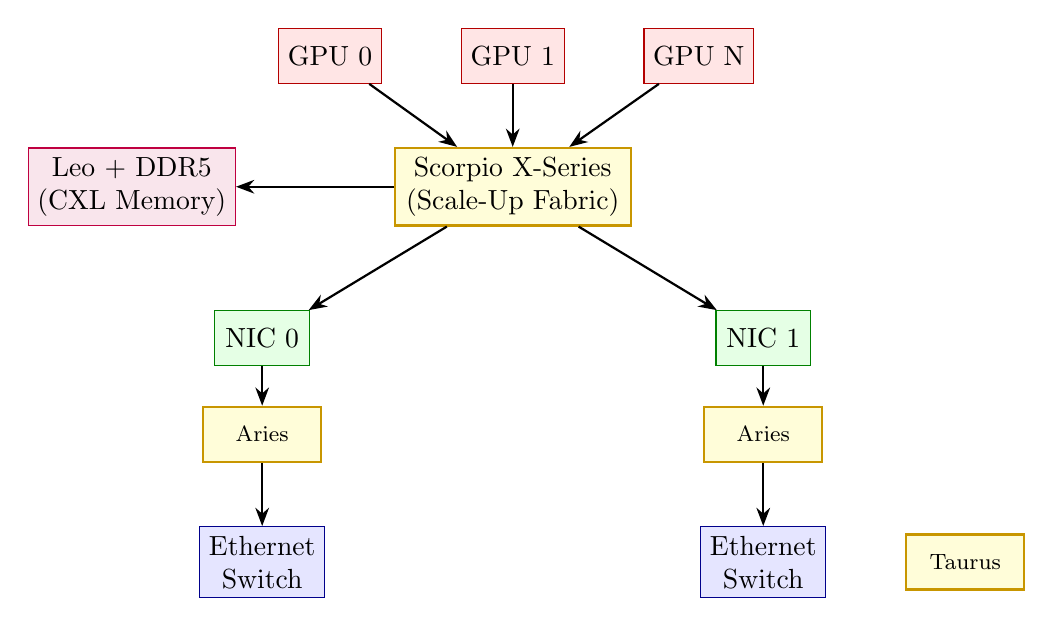
\begin{tikzpicture}[
        node distance=1.5cm and 1cm,
        gpu/.style={rectangle, draw=darkred, fill=red!10, minimum width=1.2cm, minimum height=0.7cm, align=center},
        nic/.style={rectangle, draw=darkgreen, fill=green!10, minimum width=1.2cm, minimum height=0.7cm, align=center},
        sw/.style={rectangle, draw=darkblue, fill=blue!10, minimum width=1.2cm, minimum height=0.7cm, align=center},
        ast/.style={rectangle, draw=gold, fill=yellow!15, thick, minimum width=1.5cm, minimum height=0.7cm, align=center},
        arrow/.style={->, >=Stealth, thick}
    ]
        % GPUs
        \node[gpu] (GPU1) {GPU 0};
        \node[gpu, right=of GPU1] (GPU2) {GPU 1};
        \node[gpu, right=of GPU2] (GPU3) {GPU N};

        % Scorpio between GPUs
        \node[ast, below=0.8cm of GPU2, minimum width=3cm] (SCORP) {Scorpio X-Series\\(Scale-Up Fabric)};

        % NICs
        \node[nic, below left=1.5cm of SCORP] (NIC1) {NIC 0};
        \node[nic, below right=1.5cm of SCORP] (NIC2) {NIC 1};

        % Aries
        \node[ast, below=0.5cm of NIC1, font=\footnotesize] (ARIES1) {Aries};
        \node[ast, below=0.5cm of NIC2, font=\footnotesize] (ARIES2) {Aries};

        % Ethernet fabric
        \node[sw, below=0.8cm of ARIES1] (SW1) {Ethernet\\Switch};
        \node[sw, below=0.8cm of ARIES2] (SW2) {Ethernet\\Switch};
        \node[ast, right=of SW2, font=\footnotesize] (TAURUS_N) {Taurus};

        % Memory
        \node[rectangle, draw=purple, fill=purple!10, minimum width=2cm, minimum height=0.7cm, align=center, left=2cm of SCORP] (LEO_N) {Leo + DDR5\\(CXL Memory)};

        % Arrows
        \draw[arrow] (GPU1) -- (SCORP);
        \draw[arrow] (GPU2) -- (SCORP);
        \draw[arrow] (GPU3) -- (SCORP);
        \draw[arrow] (SCORP) -- (NIC1);
        \draw[arrow] (SCORP) -- (NIC2);
        \draw[arrow] (NIC1) -- (ARIES1);
        \draw[arrow] (NIC2) -- (ARIES2);
        \draw[arrow] (ARIES1) -- (SW1);
        \draw[arrow] (ARIES2) -- (SW2);
        \draw[arrow] (SCORP) -- (LEO_N);
    \end{tikzpicture}

    \begin{itemize}
        \item \textbf{Scorpio X}：GPU-to-GPU Scale-Up（机箱/机架内）
        \item \textbf{Aries Retimer}：GPU/NIC到外部连接（背板/电缆）
        \item \textbf{Taurus}：Scale-Out网络（跨机架Ethernet）
        \item \textbf{Leo}：CXL内存扩展（GPU共享内存池）
    \end{itemize}
\end{frame}

% ============================================================
%  PART 3：Scorpio 深度研究
% ============================================================
\section{Part 3: Scorpio 深度研究}

\begin{frame}{Scorpio 产品定义}
    \begin{table}
        \caption{Scorpio 系列产品对比}
        \begin{tabular}{lll}
            \toprule
            \textbf{特性} & \textbf{Scorpio X-Series} & \textbf{Scorpio P-Series} \\
            \midrule
            定位 & Memory Semantic AI Fabric Switch & PCIe 6 Fabric Switch \\
            Lane Count & 320 lanes & 32–320 lanes \\
            协议 & Open \& Platform-Specific Memory Semantic & PCIe 6 / CXL 3.x \\
            目标应用 & GPU Scale-Up (替代/补充NVSwitch) & 通用I/O Fabric (GPU/NIC/NVMe) \\
            拓扑 & High-Radix, Single-Hop & 灵活PCIe Fabric \\
            关键特性 & HW-Accelerated Collective Ops & PCIe 6 Full Support \\
            出货状态 & 已出货至Leading Hyperscalers & 已Demo (H200+ConnectX-8) \\
            \bottomrule
        \end{tabular}
    \end{table}

    \begin{alertblock}{\textbf{本质问题：Scorpio到底是什么？}}
        \sourceT{2} 它不是传统PCIe Switch，也不是NVSwitch。它是一种\alert{新型的Fabric Switch}——基于PCIe物理层但可以运行多种协议（标准PCIe、CXL、或memory semantic的platform-specific协议）。
    \end{alertblock}
\end{frame}

\note{
    Scorpio的本质定义——这是一个关键问题：

    从技术角度看：
    - 物理层 = PCIe 6 (64 GT/s PAM4)
    - 数据链路层 = 支持标准PCIe FLIT mode，也可切换到memory semantic协议
    - 交换层 = High-radix crossbar，类似高性能网络交换机
    - 管理层 = COSMOS集成，提供per-port telemetry

    与NVSwitch的根本区别：
    - NVSwitch = 私有物理层(NVLink) + 私有协议(GPU-direct RDMA)，仅NVIDIA GPU可用
    - Scorpio = 标准物理层(PCIe) + 开放/可编程协议，任何PCIe设备可用
    - 带宽差距：NVSwitch per-GPU双向900GB/s (H100)，Scorpio per-GPU最大约128GB/s (PCIe 6 x16)
    - 这意味着：Scorpio不是为了替代NVSwitch的高性能场景，而是服务于不需要900GB/s但仍需GPU互连的场景，以及异构计算环境

    关于"320 lanes"的理解：
    - 320 lanes / 16 = 20个x16端口（如果配置为x16模式）
    - 或者可以配置为40个x8端口、80个x4端口等
    - 320 lanes是业界最大radix（公开可知的PCIe switch中），Broadcom的PEX系列最高到~144 lanes
    - 高radix = 更多设备可以直接连接（single hop），无需多级级联，降低延迟
}

\begin{frame}{为什么AI GPU集群需要Scorpio}
    \begin{columns}[T]
        \begin{column}{0.48\textwidth}
            \textbf{场景1：GPU Scale-Up Fabric}
            \begin{itemize}
                \item 多个GPU需要共享内存访问
                \item NVSwitch只连NVIDIA GPU
                \item 异构集群需要开放替代方案
                \item Custom ASIC (TPU/Trainium)需要scale-up互连
            \end{itemize}
            \vspace{0.3cm}
            \textbf{场景2：GPU-to-NIC-to-Storage}
            \begin{itemize}
                \item GPU结果需快速写入NVMe
                \item GPU需通过NIC发送到其他节点
                \item PCIe Switch消除CPU bottleneck
            \end{itemize}
        \end{column}
        \begin{column}{0.48\textwidth}
            \textbf{场景3：MoE模型通信优化}
            \begin{itemize}
                \item Mixture-of-Experts模型需要expert间all-to-all通信
                \item Scorpio的HW-accelerated collective操作减少通信延迟
                \item 官方声称提升"tokens-per-watt"\sourceT{2}
            \end{itemize}
            \vspace{0.3cm}
            \textbf{场景4：CXL内存池}
            \begin{itemize}
                \item GPU通过Scorpio访问CXL-attached DDR5内存
                \item 扩展有效内存容量（超越HBM限制）
                \item 关键：延迟 vs 容量的tradeoff
            \end{itemize}
        \end{column}
    \end{columns}
\end{frame}

\note{
    关于场景1——异构GPU集群的真实需求：
    - Google TPU v5p有8960个芯片per pod，使用Google自有的ICI (Inter-Chip Interconnect)
    - Amazon Trainium2使用AWS自有的NeuronLink
    - 但是：自研ASIC的互连技术往往不够成熟，或者成本过高
    - Scorpio提供了一个"off-the-shelf"的scale-up方案，基于成熟的PCIe生态
    - 这对中小型AI chip公司（如Cerebras、Groq、d-Matrix等）尤其有价值

    关于场景3——MoE通信优化：
    - MoE模型的每一层只有部分expert被激活（例如8个中的2个）
    - 但expert分布在不同的GPU上，需要频繁的all-to-all通信
    - 通信模式是"稀疏但大带宽"的——非常适合fabric switch
    - Caleb Shetland（Astera Sr. Principal Firmware Architect）专门写了一篇博客讨论这个问题
    - 但"tokens-per-watt"提升的具体数据未公开 \unverified
}

\begin{frame}{Scorpio vs NVSwitch 对比}
    \begin{table}
        \caption{Scorpio X-Series vs NVIDIA NVSwitch 深度对比}
        \begin{tabular}{lcc}
            \toprule
            \textbf{对比维度} & \textbf{Scorpio X-Series} & \textbf{NVIDIA NVSwitch (H100/B200)} \\
            \midrule
            物理层 & PCIe 6 (64 GT/s PAM4) & NVLink 4/5 (100/200 GT/s NRZ/PAM4) \\
            Per-GPU带宽 & ~128 GB/s (x16) & 900 GB/s (18 links × 50 GB/s) \\
            协议 & 开放 (PCIe/CXL) + Custom & 私有 (NVLink) \\
            GPU兼容 & 任何PCIe设备 & 仅NVIDIA GPU \\
            延迟 & 微秒级(推测) & <1微秒 \\
            Radix & 320 lanes (max) & 连接8 GPU (DGX), 可级联 \\
            Collective Ops & HW-Accelerated & SHARP (in-network compute) \\
            软件生态 & COSMOS & NVSwitch Fabric Manager \\
            开放vs封闭 & 开放标准+Custom & 完全私有 \\
            \bottomrule
        \end{tabular}
    \end{table}

    \begin{keypoint}
        Scorpio在\alert{绝对带宽}和\alert{延迟}上无法与NVSwitch竞争。其价值在于\alert{开放性}、\alert{异构兼容性}和\alert{高radix灵活拓扑}。
    \end{keypoint}
\end{frame}

\note{
    带宽对比深度分析：
    - NVSwitch (H100): 每个GPU有18个NVLink 4端口，每个50 GB/s双向 = 900 GB/s per GPU
    - Scorpio via PCIe 6 x16: 64 GT/s × 16 lanes = 128 GB/s per GPU（双向256 GB/s，但PCIe的编码开销约1.5%）
    - 差距约7x。但实际应用中有几个考虑：
      1. GPU的PCIe端口通常是x16，所以实际per-GPU带宽受限于PCIe root port
      2. 但在fabric中，Scorpio可以同时连接更多GPU（高radix优势）
      3. 对于只使用PCIe的非NVIDIA GPU（如AMD MI300X、Intel Gaudi 3），PCIe是唯一的scale-up选项
      4. H200的PCIe Gen5仍然是x16 64 GB/s——在PCIe时代，Scorpio的带宽匹配GPU的PCIe能力

    "Low latency"的量化问题：
    - 官方只说了"low latency"但没有给出具体数字 \unverified
    - 通过single-hop设计（高radix减少级联）降低延迟，这是真实的架构优势
    - 但PCIe switch的转发延迟通常在数百ns-数μs级别，比NVLink高1-2个数量级
    - 对于GPU scale-up（GPU直接访问远端内存），这个延迟差距是显著的限制
}

\begin{frame}{Scorpio vs Broadcom PCIe Switch}
    \begin{table}
        \caption{PCIe Fabric Switch竞争对比}
        \begin{tabular}{lcc}
            \toprule
            \textbf{维度} & \textbf{Scorpio (Astera)} & \textbf{PEX系列 (Broadcom)} \\
            \midrule
            PCIe世代 & PCIe 6 (前沿) & PCIe 5为主, 6 roadmapped \\
            最大lane数 & 320 lanes & ~144 lanes (公开) \\
            Memory Semantic & 支持 & 标准PCIe only \\
            HW Collective Ops & 支持 (Hypercast) & 未知 \\
            AI优化 & 从零为AI设计 & 通用数据中心 \\
            COSMOS集成 & 原生 & 无等效平台 \\
            市场份额 & 新进入者 & 市场领导者 \sourceT{3} \\
            Hyperscaler定制 & 积极 & 有限 \\
            成熟度/稳定性 & 较新 & 极其成熟 \\
            \bottomrule
        \end{tabular}
    \end{table}

    \begin{warningblock}
        Broadcom在PCIe Switch市场拥有十多年的积累和客户关系。Astera的进入威胁取决于Scorpio的AI特定优势是否足以抵消Broadcom的生态壁垒。
    \end{warningblock}
\end{frame}

\note{
    Broadcom的PCIe Switch护城河：
    - PEX系列（原PLX Technology, 2014年被Broadcom/Avago收购）是行业gold standard
    - 已经验证在数百万系统中，可靠性极高
    - 支持广泛的OS/BIOS/驱动生态
    - 客户（Dell, HPE, Lenovo, Supermicro等）的qualification周期长达18-24个月

    Astera的突破口：
    - PCIe 6是全新标准，所有人都在新的起跑线上
    - AI集群的特殊需求（大radix、低延迟collective ops、telemetry）不是传统PCIe switch的设计目标
    - Hyperscaler直接客户关系（不用经过OEM）缩短了qualification周期
    - 320 lanes的高radix是显著差异化（Broadcom没有公开显示类似产品）

    但风险也很明显：
    - Broadcom如果推出针对AI优化的PCIe 6 switch，其成熟的客户基础和生态会构成巨大优势
    - Astera必须在Broadcom推出竞争产品前建立足够大的客户粘性
    - 时间窗口大约是2-3年
}

\begin{frame}{Scorpio 技术架构分析}
    \centering
    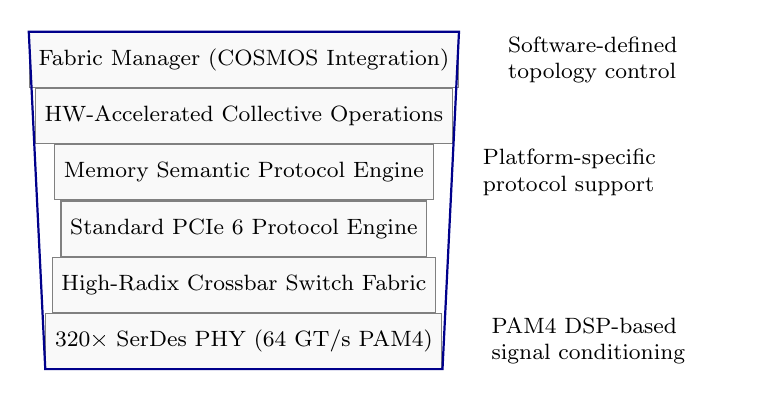
\begin{tikzpicture}[
        node distance=1cm and 2cm,
        block/.style={rectangle, draw=darkblue, fill=blue!5, thick, minimum width=2.5cm, minimum height=0.8cm, align=center, rounded corners=3pt},
        layer/.style={rectangle, draw=gray, fill=gray!5, minimum width=4cm, minimum height=0.7cm, align=center, font=\footnotesize}
    ]
        % Architecture layers
        \node[layer] (L1) {Fabric Manager (COSMOS Integration)};
        \node[layer, below=0cm of L1] (L2) {HW-Accelerated Collective Operations};
        \node[layer, below=0cm of L2] (L3) {Memory Semantic Protocol Engine};
        \node[layer, below=0cm of L3] (L4) {Standard PCIe 6 Protocol Engine};
        \node[layer, below=0cm of L4] (L5) {High-Radix Crossbar Switch Fabric};
        \node[layer, below=0cm of L5] (L6) {320× SerDes PHY (64 GT/s PAM4)};

        % Labels on the right
        \node[right=0.5cm of L1, font=\footnotesize, text width=3cm, align=left] {Software-defined\\topology control};
        \node[right=0.5cm of L3, font=\footnotesize, text width=3cm, align=left] {Platform-specific\\protocol support};
        \node[right=0.5cm of L6, font=\footnotesize, text width=3cm, align=left] {PAM4 DSP-based\\signal conditioning};

        \draw[thick, darkblue] (L1.north west) -- (L6.south west) -- (L6.south east) -- (L1.north east) -- cycle;
    \end{tikzpicture}

    \vspace{0.3cm}
    \textbf{关键技术参数（已确认）} \sourceT{2}：
    \begin{itemize}
        \item 320 SerDes lanes @ 64 GT/s PAM4（PCIe 6物理层）
        \item High-radix single-hop topology（消除多级交换的延迟叠加）
        \item HW-accelerated collective ops（All-Reduce, All-to-All等）
        \item Per-port telemetry via COSMOS
    \end{itemize}

    \textbf{未确认参数} \unverified：
    \begin{itemize}
        \item 端到端转发延迟（未公开具体ns数）
        \item 功耗（未公开W数）
        \item Die size / 制程节点（未公开，推测TSMC 7nm/5nm级别）
    \end{itemize}
\end{frame}

\note{
    关于"Memory Semantic Protocol Engine"：
    - 这是Scorpio X-Series最关键的差异化技术
    - 官方描述为支持"open and platform-specific protocols"
    - "platform-specific"意味着可能有客户定制协议——hyperscaler可以定义自己的GPU-to-GPU通信协议
    - 这种可编程性类似SmartNIC中的可编程数据平面
    - 但具体实现方式（是否使用P4/可编程pipeline/FPGA辅助）未公开

    关于"HW-Accelerated Collective Operations"（Hypercast）：
    - 类比：NVIDIA的SHARP (Scalable Hierarchical Aggregation and Reduction Protocol)
    - 在交换机内部对数据进行聚合（如All-Reduce的求和），而非全部发到端点再计算
    - 减少网络流量，降低延迟
    - 对MoE模型的All-to-All通信尤为重要
    - 但具体的性能提升数据未公开 \unverified

    关于SerDes架构：
    - 320 lanes的PAM4 SerDes是一个巨大的模拟设计挑战
    - 每个lane需要：CTLE (Continuous Time Linear Equalizer) + DFE (Decision Feedback Equalizer) + CDR + PAM4 decoder
    - 320 lanes × ~500mW per lane = ~160W仅用于SerDes（这是粗略估算）
    - 高功耗意味着需要先进的散热方案
}

\begin{frame}{Scorpio 对抗 Broadcom 的威胁评估}
    \begin{columns}[T]
        \begin{column}{0.48\textwidth}
            \textbf{Scorpio 的真实威胁}：
            \begin{enumerate}
                \item PCIe 6先行者优势——Broadcom尚未大规模出货PCIe 6 switch
                \item 320-lane高radix——超过已知的任何Broadcom产品
                \item AI-native设计——in-network computing / collective ops
                \item COSMOS统一管理——Broadcom缺乏AI优化软件
                \item Client intimacy——直接服务hyperscaler的定制需求
            \end{enumerate}
        \end{column}
        \begin{column}{0.48\textwidth}
            \textbf{Scorpio 的弱点}：
            \begin{enumerate}
                \item 未经过大规模部署验证
                \item Broadcom的客户关系和生态壁垒
                \item 缺乏传统PCIe switch的"通用"市场（企业/存储）
                \item 对AI CAPEX周期高度敏感
                \item Broadcom可以收购或自研类似方案
            \end{enumerate}
        \end{column}
    \end{columns}

    \vspace{0.3cm}
    \begin{keypoint}
        对Broadcom的威胁程度：\textbf{中等}。Scorpio主要威胁的是AI-specific的增量市场，而非Broadcom的传统企业/存储switch业务。但AI market的增速远超传统市场。
    \end{keypoint}
\end{frame}

\note{
    威胁评估的深入分析：

    短期（1-2年）：
    - Scorpio在AI GPU集群领域几乎没有直接竞争对手（除了NVIDIA NVSwitch）
    - Broadcom的PCIe 6 switch roadmapped但未大规模出货
    - 时间窗口有利于Astera

    中期（2-4年）：
    - Broadcom肯定会推出AI-optimized PCIe 6 switch
    - 但Broadcom的服务模式（通过OEM间接服务hyperscaler）vs Astera的直接服务模式可能是持久差异
    - 关键变量：hyperscaler是否愿意将PCIe switch也multi-source

    长期（4年+）：
    - 如果PCIe-based fabric成为AI集群主流，Broadcom和Microchip都会进入
    - 潜在的新进入者：NVIDIA可能自己出PCIe switch来绑定其GPU
    - Astera的护城河需要从"先发优势"进化为"生态锁定"（COSMOS是关键）

    Scorpio对Broadcom具体业务的影响：
    - Broadcom FY2024 networking revenue ~$30B+（包括Ethernet switch等）
    - 其中PCIe switch只占一小部分（估计$1-2B级别）
    - 所以Scorpio对Broadcom整体业务影响有限
    - 但AI PCIe switch是Broadcom增长最快的细分市场之一
}

\begin{frame}{Scorpio 的护城河与真实价值}
    \textbf{护城河评估}：

    \begin{table}
        \begin{tabular}{lcc}
            \toprule
            \textbf{壁垒} & \textbf{强度} & \textbf{说明} \\
            \midrule
            High-Speed SerDes & \checkmark\checkmark\checkmark & 320-lane 64GT/s PAM4是极高难度的模拟设计 \\
            Hyperscaler Qualification & \checkmark\checkmark\checkmark & 已通过hyperscaler的严格验证并出货 \\
            Memory Semantic Protocol & \checkmark\checkmark & 可编程协议引擎，但其他厂商可模仿 \\
            COSMOS Integration & \checkmark\checkmark & 软件差异化，但客户可能自研管理工具 \\
            Ecosystem Lock-in & \checkmark & 仍处于建立阶段，锁定效应弱 \\
            \bottomrule
        \end{tabular}
    \end{table}

    \vspace{0.2cm}
    \textbf{Scorpio 在 AI Infra 中的真实价值}：

    \begin{itemize}
        \item 目前是唯一基于PCIe并针对AI优化的大radix fabric switch
        \item 解决了异构GPU环境的scale-up互连问题（非NVIDIA GPU的核心需求）
        \item 为hyperscaler提供了NVIDIA之外的战略性替代方案
        \item 但其性能天花板（PCIe带宽/延迟）限制了在最高性能场景的适用性
    \end{itemize}
\end{frame}

\note{
    护城河深度分析：

    SerDes壁垒（最真实）：
    - 320 lane的64GT/s PAM4 SerDes集成在一个芯片上是一个极大的模拟工程挑战
    - PAM4的信噪比要求远高于NRZ（PAM4有4个电平，NRZ只有2个）
    - Crosstalk management在320 lane的密度下极其困难
    - 这是真正的技术壁垒——并非每个公司都能做

    Hyperscaler Qualification壁垒（真实但可被复制）：
    - Hyperscaler的qualification包括：热冲击测试、加速老化测试、FIT rate验证、电源噪声测试、系统级互操作测试
    - 周期长达12-24个月
    - 一旦通过，更换供应商的成本很高（需要重新qualify）
    - 但这只是时间壁垒，不是技术壁垒——竞争对手有足够资金和时间也能通过

    Memory Semantic Protocol壁垒（中等）：
    - 可编程协议引擎增加了灵活性，但不一定是强锁定
    - 如果竞争对手支持标准CXL 3.x（也支持memory semantic），功能会趋同
    - 主要的差异化在于和客户共同定制的"platform-specific"协议——这部分是保密的

    COSMOS Integration壁垒（中等偏弱）：
    - 统一管理的价值真实存在，但hyperscaler自己也可以开发管理工具
    - 对于有强大软件能力的hyperscaler（Google、Amazon），这不一定是壁垒
    - 对于软件能力较弱的客户，COSMOS的"开箱即用"价值更高

    总结：Astera Labs的护城河是真实的，但最坚固的部分（SerDes、Qualification）是时间性的而非永久性的。公司需要在时间窗内最大化客户采用和生态锁定。
}

\end{document}
